\section{Projektplanung}
\label{sec:project_plan}
Abbildung \ref{fig:workpackages} zeigt die Aufteilung Masterthesis in einzelne Arbeitspakete. Das Ziel der Einarbeitungsphase ist ein grundlegendes Verständnis über die Datenverarbeitung im Hadoop-Framework zu erhalten. Zusätzlich soll eine Entwicklungsumgebung inklusive öffentlicher Versionsverwaltung eingerichtet werden. Darauf erfolgt der Aufbau eines eigenen Hadoop-Clusters und die Beschaffung von Testdaten.\footnote{Auch ein Zugriff auf einen bestehendes Hadoop-Cluster ist möglich.} Für die Einarbeitung und den Aufbau sind vier Wochen eingeplant (siehe Abbildung \ref{fig:ganttA}).\footnote{Die referenzierten Gantt-Diagramme wurden mit der JavaScript-Bibliothek \textit{dhtmlxGantt} erstellt. Der Quellcode ist unter der \textit{GNU GPLv2}-Lizenz lizenziert. Weiter Informationen können in Kapitel \ref{sec:licencing_issues} im Anhang nachgelesen werden.}\\

\noindent
Der zweite Teil behandelt die Rohdatenspeicherung im HDFS und eine Datenaufbereitung. Es soll geprüft werden, welche Struktur der Daten für eine optimale Speicherung und Verarbeitung im Hadoop-Framework erforderlich ist. Dieser Teil beansprucht abermals vier Wochen. Am Ende dieses Arbeitspaketes soll ein erster Zwischenbericht erstellt werden, welcher die bisherigen Ergebnisse enthält (sieh Abbildung \ref{fig:ganttA}).\\

\begin{figure}[ht]
  \centering
  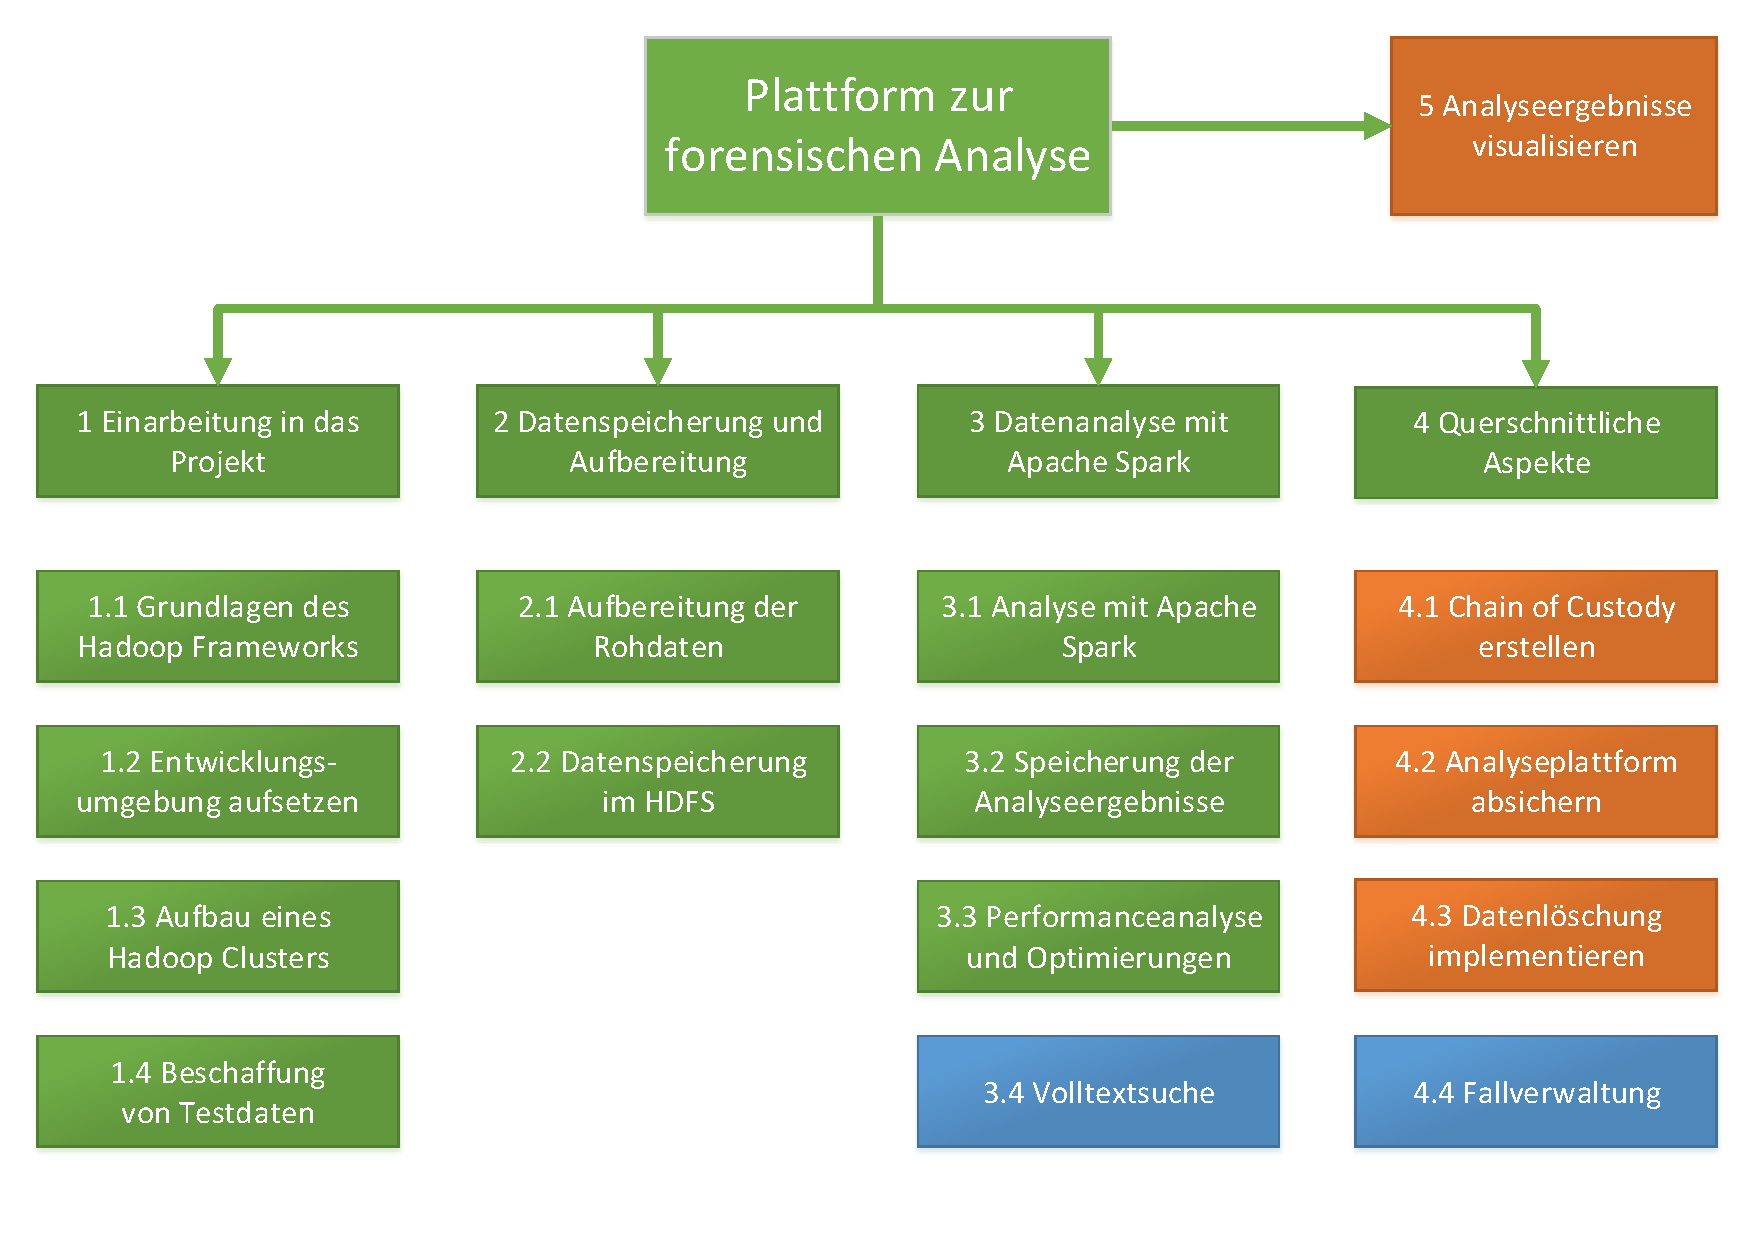
\includegraphics[width=\textwidth]{./resource/Arbeitspakete.pdf}
  \caption{Arbeitspakete der Masterthesis}
  \label{fig:workpackages}
\end{figure}

\noindent
Nach der Speicherung der Rohdaten erfolgt im dritten Arbeitspaket die Datenanalyse mit Apache Spark. Hier sollen die Daten nach anwendungsbezogenen Problemstellungen analysiert werden. Das Ergebnis ist eine Sammlung von Programmen, welche mit Apache Spark auf den Daten ausgeführt werden können. Darüber hinaus soll ermittelt werden, welche Möglichkeiten zur Ausführung dieser Spark-Anwendungen bestehen.\footnote{Hier könnte beispielsweise das Projekt Apache Livy nützlich sein.} Ein weiterer Aspekt der Datenanalyse beschäftigt sich mit den Möglichkeiten, wie die Ergebnisse persistiert werden können.\footnote{Hier könnten die
Projekte Apache Hive und Apache HBase zur Speicherung von strukturierten und unstrukturierten Daten untersucht werden.} Im Anschluss soll die Performanz der Algorithmen geprüft werden. Hier bietet sich der Vergleich zu herkömmlichen Analyseprogrammen an. Denn schließlich hat diese Thesis auch das Ziel, bei großen Datenmengen schneller Ergebnisse zu liefern als die herkömmlichen Analysewerkzeuge auf einem einzelnen Analyserechner. Für dieses Arbeitspaket sind sieben Wochen eingeplant (siehe Abbildung \ref{fig:ganttB}). Darauf folgt ein zweiter Zwischenbericht.\\

\noindent
Im letzten Drittel der Masterthesis sollen die querschnittlichen Aspekte in der bestehenden Datenverarbeitung berücksichtigt werden. Hierbei geht es um das Absichern der Analyseplattform, die Dokumentation der Chain of Custody und das Löschen von nicht mehr verwendeten personenbezogenen Daten. Für dieses Arbeitspaket sind vier Wochen eingeplant (siehe Abbildung \ref{fig:ganttC}).\\

\noindent
Das letzte Arbeitspaket enthält ein prototypische Visualisierung der Analyseergebnisse. Hierbei soll geprüft werden, welche Möglichkeiten zur Darstellung der Ergebnisse existieren. Der Forensiker soll auf möglichst einfache Art und Weise die Ergebnisse ansehen können. Für diese Arbeit sind drei Wochen eingeplant (siehe Abbildung \ref{fig:ganttC}).\\

\begin{figure}[p]
  \centering
  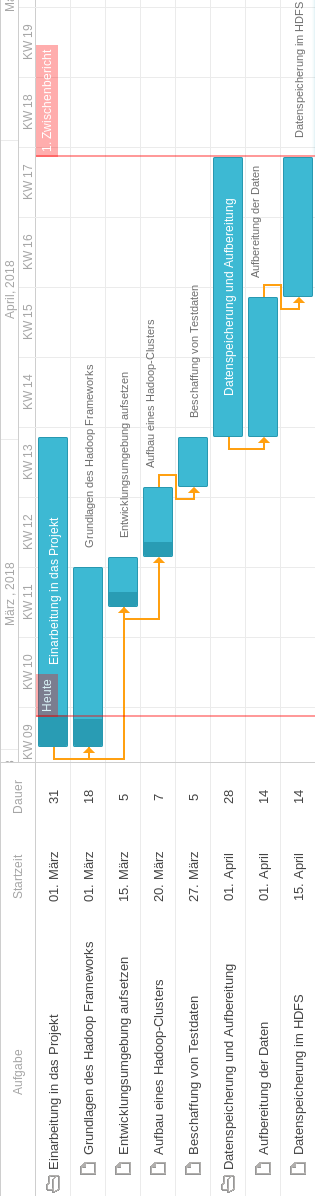
\includegraphics[width=\textwidth,height=\textheight,keepaspectratio]{./resource/ganttA.png}
  \caption{Projektplan Teil A - Einarbeitung und Rohdatenspeicherung (siehe Kapitel \ref{sec:licencing_issues})}
  \label{fig:ganttA}
\end{figure}

\begin{figure}[p]
  \centering
  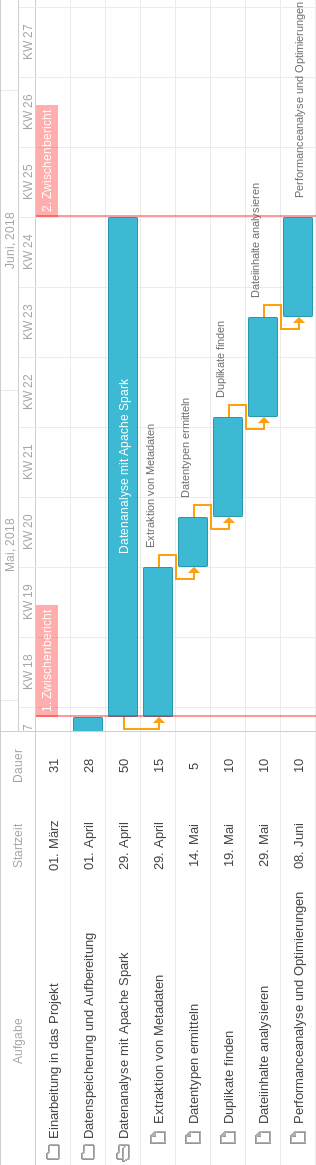
\includegraphics[width=\textwidth,height=\textheight,keepaspectratio]{./resource/ganttB.png}
  \caption{Projektplan Teil B - Datenanalyse (siehe Kapitel \ref{sec:licencing_issues})}
  \label{fig:ganttB}
\end{figure}

\begin{figure}[p]
  \centering
  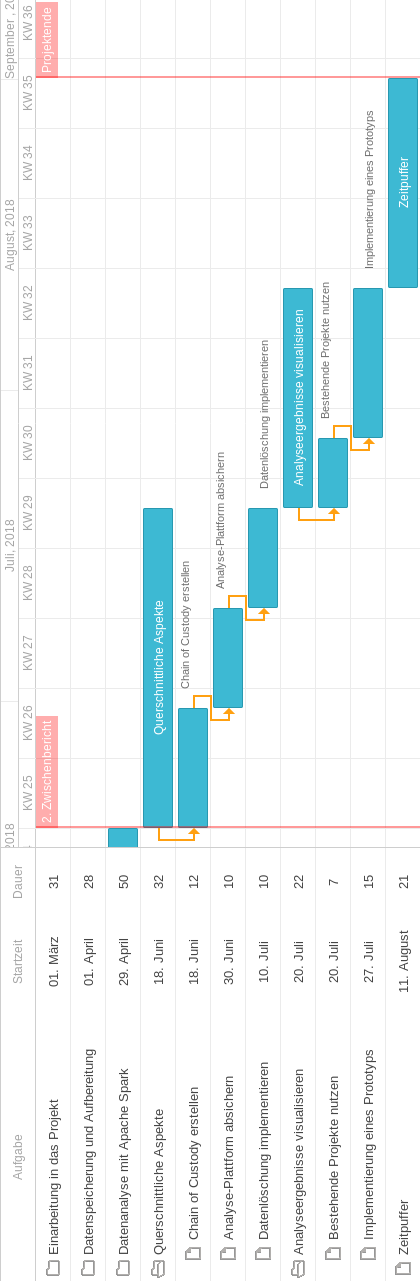
\includegraphics[width=\textwidth,height=\textheight,keepaspectratio]{./resource/ganttC.png}
  \caption{Projektplan Teil C - Querschnittliche Aspekte und Visualisierung (siehe Kapitel \ref{sec:licencing_issues})}
  \label{fig:ganttC}
\end{figure}

\clearpage
\section{Entwicklungsumgebung}
\label{development_environment}
Der Aufbau eine Test- und Entwicklungsumgebung ist ein essentieller Bestandteil dieser Thesis. Einerseits sollen Anwendungsprogramme zur Datenverarbeitung schnell und lokal ausführbar sein und andererseits, soll die Testumgebung auf einem physikalisches Apache Hadoop Cluster laufen, um mögliche Infrastrukturproblem identifizieren zu können. \\

\noindent
Alle selbst erstellten Anwendungsprogramme, Konfigurationsdateien und die Dokumentation dieser Thesis sollen als Open Source - Quelle in einem öffentlichen Repository zugänglich sein. Aus fachlicher Sicht ist es gerade in der Forensik sehr wichtig, dem Nutzer die Möglichkeit zu geben, den Quellcode der Analyseprogramme einsehen zu können und in notfalls auf spezielle Bedürfnisse anzupassen. Darüber hinaus kann die Datenverarbeitung transparent nachvollzogen werden.\\

\noindent
Aus diesem Grund soll sämtlicher Source-Code unter der Apache License vertrieben werden. Es soll jedem möglich sein, die Dateien einzusehen. Darüber hinaus wird das Projekt vorerst unter GitHub gehostet.
